\documentclass[tikz]{standalone}
\usetikzlibrary{decorations.pathreplacing,decorations.pathmorphing,calc}
\tikzset{
	source/.pic = {
		\draw (0.5, 0.7) -- ++(0, -0.2) --
		      ++(-0.5, 0) -- ++(0, 0.5) --
		      ++(-0.7, 0) -- ++(0, -2) --
		      ++(0.7, 0) -- ++(0, 0.5) --
		      ++(0.5, 0) -- ++(0, -0.2);
	},
	detector/.pic = {
		\draw [fill=gray] (-1, 1) rectangle (1, -1);
		\draw (-0.8, 1) -- ++(0, -2);
	},
	slab/.pic = {
		\draw [fill=gray!50] (-0.2, 2) rectangle (0.2, -2);
	},
	human/.pic = {
		\draw [fill=gray] (0, 0) 
		.. controls ++(180:-1) and ++(-90: 1) .. ( 2, 1)
		.. controls ++(-90:-1) and ++(180:-1) .. ( 0, 2)
		.. controls ++(180: 1) and ++(-90:-1) .. (-2, 1)
		.. controls ++(-90: 1) and ++(180: 1) .. ( 0, 0);
		\draw [fill=white] (0, 1.5) ellipse (0.8 and 1);
		\draw (-.1, 2.49) to [in=180, out=30] ++(0.1, 0.2) to [in=150, out=0] ++(0.1, -0.2);
		\path[thick, fill=white] (-.1, 2.48) to [in=180, out=30] ++(0.1, 0.2) to [in=150, out=0] ++(0.1, -0.2) --cycle;
	}
}

\def\centerarc[#1](#2)(#3:#4:#5)% Syntax: [draw options] (center) (initial angle:final angle:radius)
    { \draw[#1] ($(#2)+({#5*cos(#3)},{#5*sin(#3)})$) arc (#3:#4:#5); }
\definecolor{photoncolor}{rgb}{0.65, 0.16, 0.16}
\begin{document}
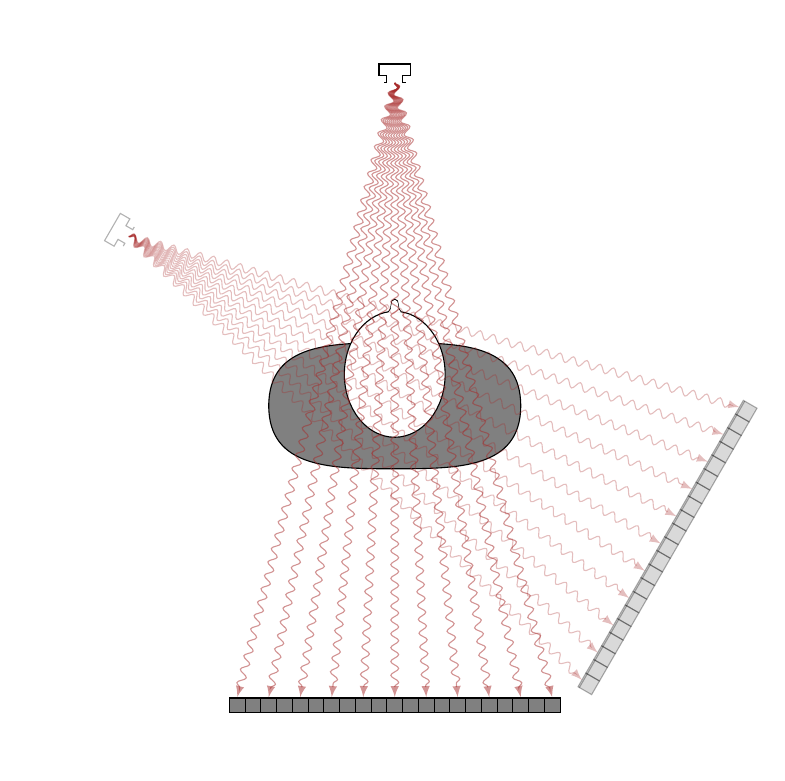
\begin{tikzpicture}
	\pic[scale=0.8] at (0,-1) {human};
	\def\opa{0.4}
	\pic[transform shape, local bounding box=source, rotate=-90, scale=0.2] at (0, 4) {source};
	\foreach [count=\i] \minoroff in {-2,-1.8,...,2}
	{
		\pic[transform shape, local bounding box=detector, rotate=-90,scale=0.1] at (0+\minoroff, -4) {detector};
		\ifodd\i \draw [
			-latex, decorate, decoration={snake, amplitude=0.05cm, segment length=5pt, post length=1mm},%
			color=photoncolor, opacity=0.5
			] (source.south) -- (detector.north);\fi
	}
	\centerarc[-latex, thick, dashed](0,0)(95:145:4);
	\rotatebox{60}{
		\pic[rotate=-90,opacity=0.3, local bounding box=source, scale=0.2] at (0, 4) {source};
		\foreach [count=\i] \minoroff in {-2,-1.8,...,2}
		{
			\pic[transform shape, opacity=0.3, local bounding box=detector, rotate=-90,scale=0.1] at (\minoroff, -4) {detector};
			\ifodd\i\draw [
				-latex, decorate, decoration={snake, amplitude=0.05cm, segment length=5pt, post length=1mm},%
				color=photoncolor, opacity=0.3
				] (source.south) -- (detector.north);\fi
		}
	}
	\begin{scope}[rotate=45,opacity=0]
	\foreach \xoff in {-2.3, 2.3}
	{
		\pic[rotate=-90,opacity=0, local bounding box=source, scale=0.2] at (\xoff, 4) {source};
		\pic[rotate=-90,transform shape, opacity=0, local bounding box=detector, scale=0.1] at (\xoff, -4) {detector};
		\draw [
			-latex, decorate, decoration={snake, amplitude=0.05cm, segment length=5pt, post length=1mm},%
			color=photoncolor, opacity=0
		] (source.south) -- (detector.north);%
	}
	\end{scope}
\end{tikzpicture}
\end{document}
